
\color{black}
\subsection*{fitting a self organizing map to in-game data}
The file \texttt{q3dm1-path2.csv} contains a sequence 
\begin{equation*}
\vec{x}[1]:\vec{x}[2]:\vec{x}[3]:\vec{x}[3]:\cdots:\vec{x}[n]
\end{equation*}
of 3D locations the avatar of a human player was seen at while moving around the Quake III map \textit{q3dm1}. When plotted, these data look like this
\begin{center}
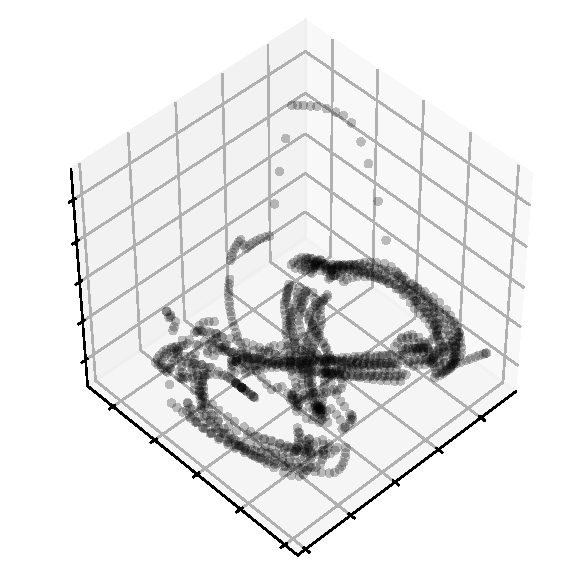
\includegraphics[width=0.75\textwidth]{q3dm1-data-path2.pdf}
\end{center}

Fit a self organizing map of $k=24$ neurons into the given data points $\vec{x}[t]$. This SOM should have the following topological- or \emph{map space} structure
\begin{center}
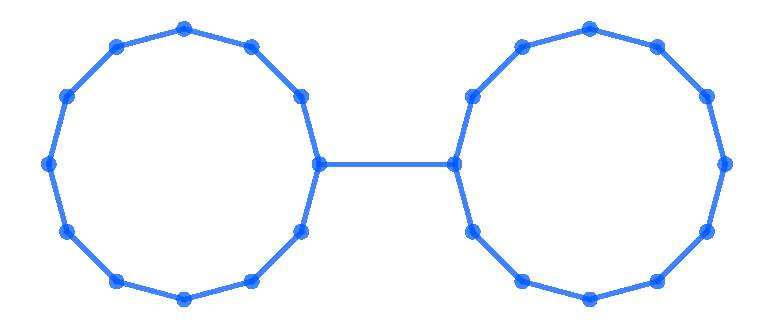
\includegraphics[width=0.6\textwidth]{som-infty-topology.pdf}
\end{center}
\newpage





Plot the data in \texttt{q3dm1-path2.csv} together with the SOM you fitted to it. Plot data points in black and SOM weights and their connections in \textcolor{blue}{blue}.

\textbf{Note:} if your fitted SOM looks ``twisted'', then run the training algorithm again, until you obtain a better fit.
%%%%%
%%%%% enter your answer here, i.e. replace "placeholder.pdf" by the name of the graphics file you created
%%%%%
\begin{center}

\includegraphics[width=0.5\textwidth]{placeholder.pdf}
\end{center}
%%%%%
%%%%%
%%%%%





\vspace{2cm}
Once you have fitted your SOM, determine how well its weights $\vec{w}_1, \ldots, \vec{w}_k$ represent the data. To do this, compute the mean squared error
\begin{equation*}
E = \frac{1}{n} \sum_{t=1}^n \, \min_i \, \dsq{\vec{x}[t]}{\vec{w}_i}
\end{equation*}
Round your result to \emph{two} decimals and enter it here \color{blue}
%%%%%
%%%%% enter your answer after the '=' sign
%%%%%
\begin{equation*}
E = 
\end{equation*}
%%%%%
%%%%%
%%%%%
%%%%%
\color{black}
\newpage